\documentclass{../ape}

\usepackage{../../linma2345}

\begin{document}

\session{7}{Sequential Equilibria}

\section{}
Using the game in extensive form below, show that it is not possible to find the Nash equilibria (in mixed strategies) by only computing the equilibria of the multi-agent representation (where each decision state is assumed to be a different player).

\begin{center}
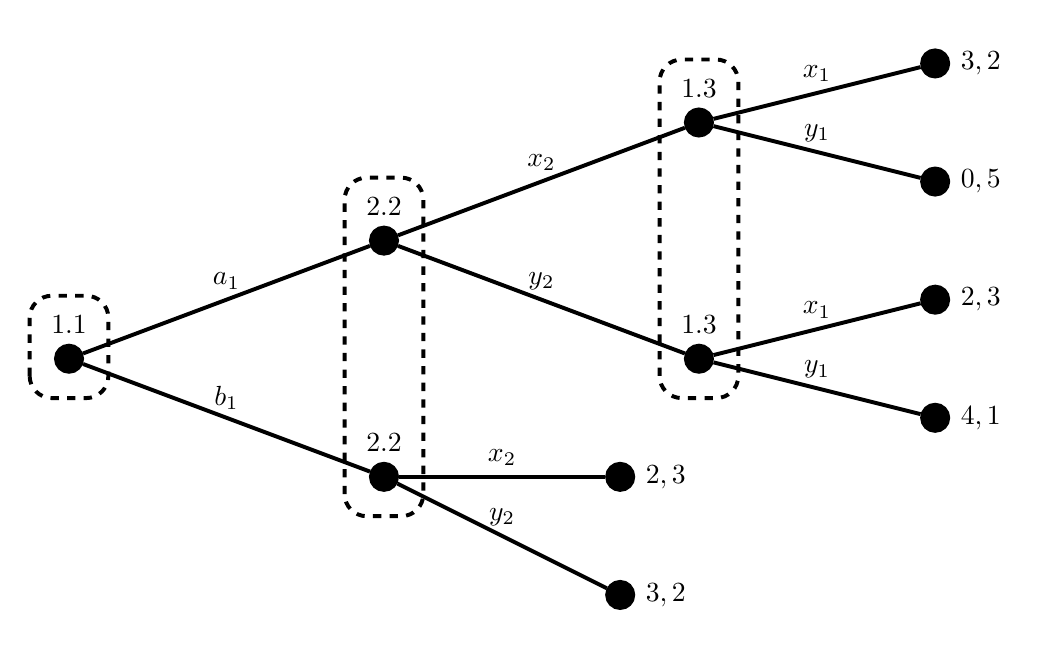
\begin{tikzpicture}[scale=2,looseness=.8,auto]
	\begin{scope}[every node/.style={font=\small\itshape},line width=0.5mm]
		\tikzstyle{every node}=[draw,fill=black,shape=circle,line width=0.5mm,minimum size=1.5mm,label distance=1mm];
		\path (0, 0   ) node (v11)  {} node [above,draw=none,fill=none] {$1.1$};
		\path (2, 0.75) node (v22a) {} node [above,draw=none,fill=none] {$2.2$};
		\path (2,-0.75) node (v22b) {} node [above,draw=none,fill=none] {$2.2$};
		\path (4, 1.5 ) node (v13a) {} node [above,draw=none,fill=none] {$1.3$};
		\path (4, 0   ) node (v13b) {} node [above,draw=none,fill=none] {$1.3$};
		\path (5.5, 1.875) node (po1) {} node [right,draw=none,fill=none,xshift=1mm] {$3,2$};
		\path (5.5, 1.125) node (po2) {} node [right,draw=none,fill=none,xshift=1mm] {$0,5$};
		\path (5.5, 0.375) node (po3) {} node [right,draw=none,fill=none,xshift=1mm] {$2,3$};
		\path (5.5,-0.375) node (po4) {} node [right,draw=none,fill=none,xshift=1mm] {$4,1$};
		\path (3.5,-0.75 ) node (po5) {} node [right,draw=none,fill=none,xshift=1mm] {$2,3$};
		\path (3.5,-1.5  ) node (po6) {} node [right,draw=none,fill=none,xshift=1mm] {$3,2$};
		\draw (v11)  -- (v22a) node [midway,above,draw=none,fill=none,yshift=-1.5mm] {$a_1$};
		\draw (v11)  -- (v22b) node [midway,above,draw=none,fill=none,yshift=-1.5mm] {$b_1$};
		\draw (v22a) -- (v13a) node [midway,above,draw=none,fill=none,yshift=-1.5mm] {$x_2$};
		\draw (v22a) -- (v13b) node [midway,above,draw=none,fill=none,yshift=-1.5mm] {$y_2$};
		\draw (v13a) -- (po1)  node [midway,above,draw=none,fill=none,yshift=-1.5mm] {$x_1$};
		\draw (v13a) -- (po2)  node [midway,above,draw=none,fill=none,yshift=-1.5mm] {$y_1$};
		\draw (v13b) -- (po3)  node [midway,above,draw=none,fill=none,yshift=-1.5mm] {$x_1$};
		\draw (v13b) -- (po4)  node [midway,above,draw=none,fill=none,yshift=-1.5mm] {$y_1$};
		\draw (v22b) -- (po5)  node [midway,above,draw=none,fill=none,yshift=-1.5mm] {$x_2$};
		\draw (v22b) -- (po6)  node [midway,above,draw=none,fill=none,yshift=-1.5mm] {$y_2$};
		
		\draw[rounded corners=8pt,dashed] (-.25,-.25) rectangle (0.25,0.4);
		\draw[rounded corners=8pt,dashed] (1.75,-1) rectangle (2.25,1.15);
		\draw[rounded corners=8pt,dashed] (3.75,-.25) rectangle (4.25,1.9);
	\end{scope}
\end{tikzpicture}
\end{center}

\nosolution

\section{}
Consider the following game in extensive form and the following scenario:

\begin{center}
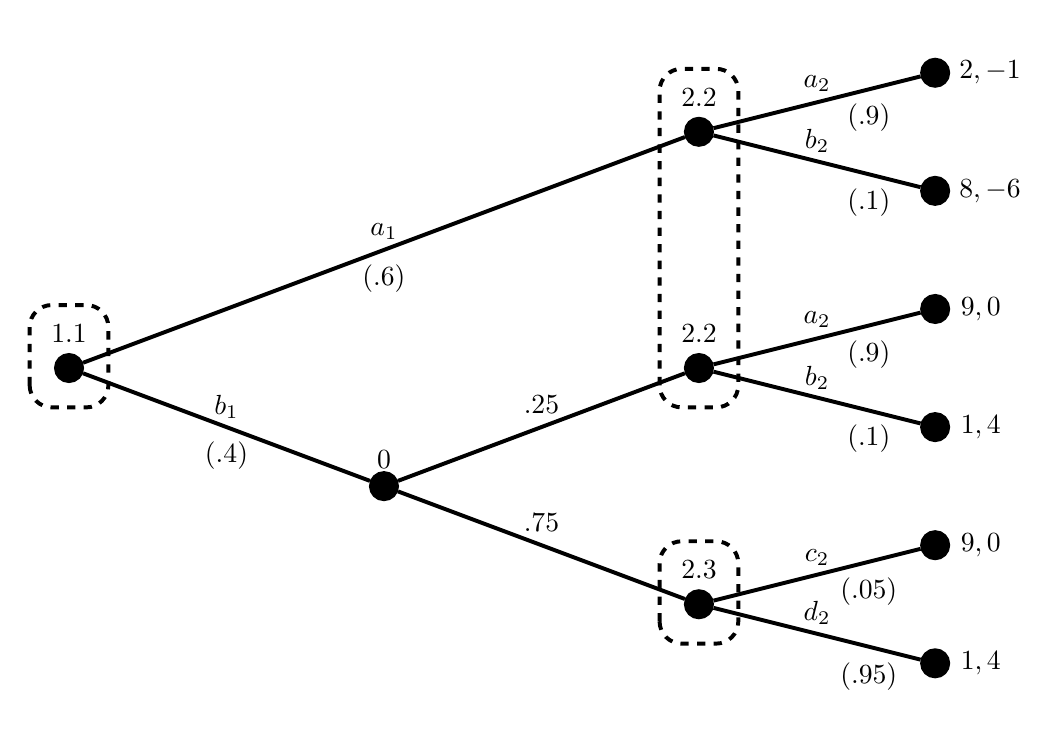
\begin{tikzpicture}[scale=2,looseness=.8,auto]
	\begin{scope}[every node/.style={font=\small\itshape},line width=0.5mm]
		\tikzstyle{every node}=[draw,fill=black,shape=circle,line width=0.5mm,minimum size=1.5mm,label distance=1mm];
		\path (0, 0   ) node (v11)  {} node [above,draw=none,fill=none] {$1.1$};
		\path (2,-0.75) node (v0)   {} node [above,draw=none,fill=none] {$0$};
		\path (4, 1.5 ) node (v22a) {} node [above,draw=none,fill=none] {$2.2$};
		\path (4, 0   ) node (v22b) {} node [above,draw=none,fill=none] {$2.2$};
		\path (4,-1.5 ) node (v23)  {} node [above,draw=none,fill=none] {$2.3$};
		\path (5.5, 1.875) node (po1) {} node [right,draw=none,fill=none,xshift=1mm] {$2,-1$};
		\path (5.5, 1.125) node (po2) {} node [right,draw=none,fill=none,xshift=1mm] {$8,-6$};
		\path (5.5, 0.375) node (po3) {} node [right,draw=none,fill=none,xshift=1mm] {$9,0$};
		\path (5.5,-0.375) node (po4) {} node [right,draw=none,fill=none,xshift=1mm] {$1,4$};
		\path (5.5,-1.125) node (po5) {} node [right,draw=none,fill=none,xshift=1mm] {$9,0$};
		\path (5.5,-1.875) node (po6) {} node [right,draw=none,fill=none,xshift=1mm] {$1,4$};
		\draw (v11)  -- (v22a) node [midway,above,draw=none,fill=none,yshift=-1.5mm] {$a_1$} node [midway,below,draw=none,fill=none,yshift=1.5mm] {$(.6)$};
		\draw (v11)  -- (v0)   node [midway,above,draw=none,fill=none,yshift=-1.5mm] {$b_1$} node [midway,below,draw=none,fill=none,yshift=1.5mm] {$(.4)$};
		\draw (v0)   -- (v22b) node [midway,above,draw=none,fill=none,yshift=-1.5mm] {$.25$};
		\draw (v0)   -- (v23)  node [midway,above,draw=none,fill=none,yshift=-1.5mm] {$.75$};
		\draw (v22a) -- (po1)  node [midway,above,draw=none,fill=none,yshift=-1.5mm] {$a_2$} node [near end,below,draw=none,fill=none,yshift=1.5mm] {$(.9)$};
		\draw (v22a) -- (po2)  node [midway,above,draw=none,fill=none,yshift=-1.5mm] {$b_2$} node [near end,below,draw=none,fill=none,yshift=1.5mm] {$(.1)$};
		\draw (v22b) -- (po3)  node [midway,above,draw=none,fill=none,yshift=-1.5mm] {$a_2$} node [near end,below,draw=none,fill=none,yshift=1.5mm] {$(.9)$};
		\draw (v22b) -- (po4)  node [midway,above,draw=none,fill=none,yshift=-1.5mm] {$b_2$} node [near end,below,draw=none,fill=none,yshift=1.5mm] {$(.1)$};
		\draw (v23)  -- (po5)  node [midway,above,draw=none,fill=none,yshift=-1.5mm] {$c_2$} node [near end,below,draw=none,fill=none,yshift=2mm] {$(.05)$};
		\draw (v23)  -- (po6)  node [midway,above,draw=none,fill=none,yshift=-1.5mm] {$d_2$} node [near end,below,draw=none,fill=none,yshift=2mm] {$(.95)$};
		
		\draw[rounded corners=8pt,dashed] (-.25,-.25) rectangle (0.25,0.4);
		\draw[rounded corners=8pt,dashed] (3.75,-.25) rectangle (4.25,1.9);
		\draw[rounded corners=8pt,dashed] (3.75,-1.75) rectangle (4.25,-1.1);
	\end{scope}
\end{tikzpicture}
\end{center}

\begin{enumerate}
	\item[a.] Compute belief probabilities that are consistent with this scenario.
	\item[b.] For each player, at each of his information state, compute the sequential value of each available actions. We here keep the same scenario and we will use the belief probabilities found at question a.
	\item[c.] Identify all the irrational actions in this scenario and with these belief probabilities (that is to say, for each information state of each player, identify all the actions that have a non-zero probability of being selected but that do not maximize the sequential value in this information state).
	\item[d.] Find a sequential equilibrium for this game.
\end{enumerate}

\nosolution

\section{}
Consider the following game in extensive form:

\begin{center}
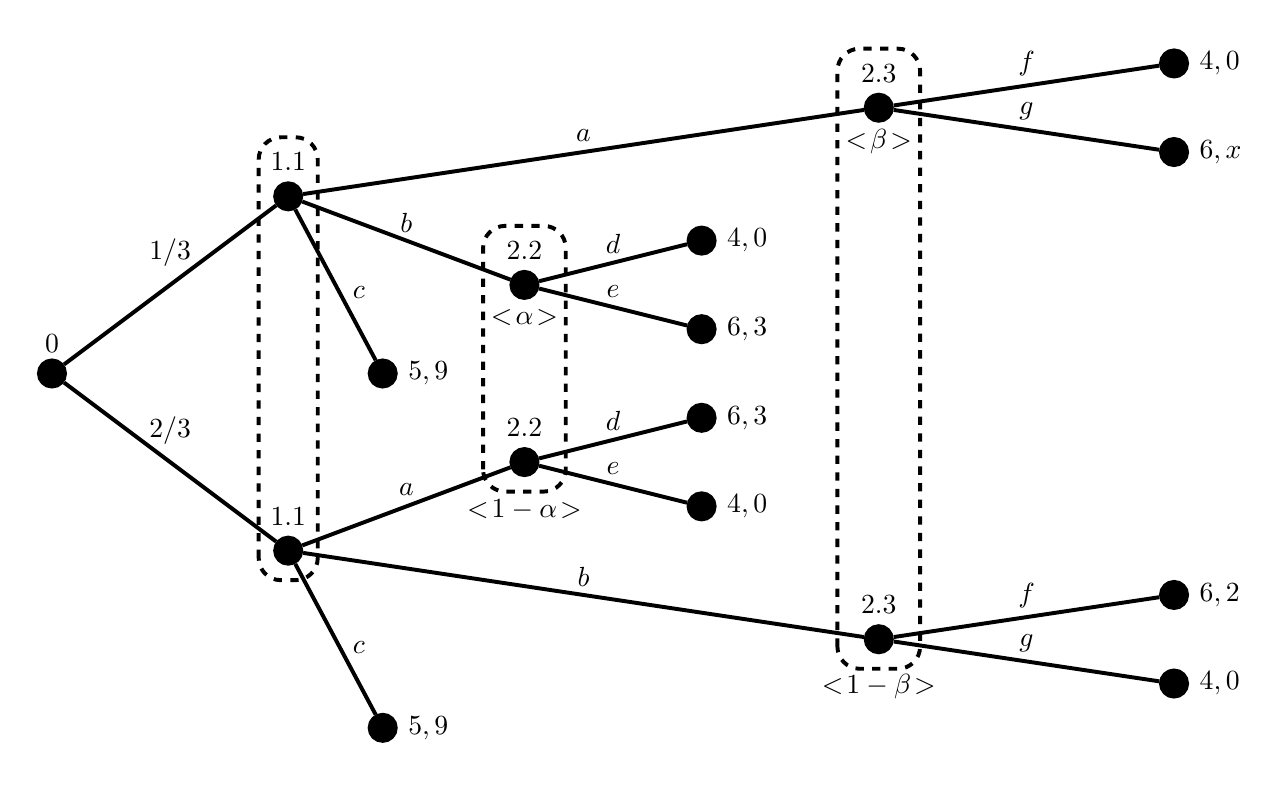
\begin{tikzpicture}[scale=1.5,looseness=.8,auto]
	\begin{scope}[every node/.style={font=\small\itshape},line width=0.5mm]
		\tikzstyle{every node}=[draw,fill=black,shape=circle,line width=0.5mm,minimum size=1.5mm,label distance=1mm];
		\path (0, 0   ) node (v0)   {} node [above,draw=none,fill=none,yshift=.5mm] {$0$};
		\path (2, 1.5 ) node (v11a) {} node [above,draw=none,fill=none] {$1.1$};
		\path (2,-1.5 ) node (v11b) {} node [above,draw=none,fill=none] {$1.1$};
		\path (4, 0.75) node (v22a) {} node [above,draw=none,fill=none] {$2.2$} node [below,draw=none,fill=none,yshift=2mm] {$<\!\alpha\!>$};
		\path (4,-0.75) node (v22b) {} node [above,draw=none,fill=none] {$2.2$} node [below,draw=none,fill=none,yshift=3mm] {$<\!1-\alpha\!>$};
		\path (7, 2.25) node (v23a) {} node [above,draw=none,fill=none] {$2.3$} node [below,draw=none,fill=none,yshift=2mm] {$<\!\beta\!>$};
		\path (7,-2.25) node (v23b) {} node [above,draw=none,fill=none] {$2.3$} node [below,draw=none,fill=none,yshift=3mm] {$<\!1-\beta\!>$};
		\path (2.8, 0    ) node (po1) {} node [right,draw=none,fill=none,xshift=1mm] {$5,9$};
		\path (2.8,-3    ) node (po2) {} node [right,draw=none,fill=none,xshift=1mm] {$5,9$};
		\path (5.5, 1.125) node (po3) {} node [right,draw=none,fill=none,xshift=1mm] {$4,0$};
		\path (5.5, 0.375) node (po4) {} node [right,draw=none,fill=none,xshift=1mm] {$6,3$};
		\path (5.5,-0.375) node (po5) {} node [right,draw=none,fill=none,xshift=1mm] {$6,3$};
		\path (5.5,-1.125) node (po6) {} node [right,draw=none,fill=none,xshift=1mm] {$4,0$};
		\path (9.5, 2.625) node (po7) {} node [right,draw=none,fill=none,xshift=1mm] {$4,0$};
		\path (9.5, 1.875) node (po8) {} node [right,draw=none,fill=none,xshift=1mm] {$6,x$};
		\path (9.5,-1.875) node (po9) {} node [right,draw=none,fill=none,xshift=1mm] {$6,2$};
		\path (9.5,-2.625) node (po0) {} node [right,draw=none,fill=none,xshift=1mm] {$4,0$};
		\draw (v0)   -- (v11a) node [midway,above,draw=none,fill=none,yshift=-1mm] {$1/3$};
		\draw (v0)   -- (v11b) node [midway,above,draw=none,fill=none,yshift=-1mm] {$2/3$};
		\draw (v11a) -- (v22a) node [midway,above,draw=none,fill=none,yshift=-1mm] {$b$};
		\draw (v11a) -- (v23a) node [midway,above,draw=none,fill=none,yshift=-1mm] {$a$};
		\draw (v11b) -- (v22b) node [midway,above,draw=none,fill=none,yshift=-1mm] {$a$};
		\draw (v11b) -- (v23b) node [midway,above,draw=none,fill=none,yshift=-1mm] {$b$};
		\draw (v11a) -- (po1)  node [midway,above,right,draw=none,fill=none,yshift=-1mm] {$c$};
		\draw (v11b) -- (po2)  node [midway,above,right,draw=none,fill=none,yshift=-1mm] {$c$};
		\draw (v22a) -- (po3)  node [midway,above,draw=none,fill=none,yshift=-1mm] {$d$};
		\draw (v22a) -- (po4)  node [midway,above,draw=none,fill=none,yshift=-1mm] {$e$};
		\draw (v22b) -- (po5)  node [midway,above,draw=none,fill=none,yshift=-1mm] {$d$};
		\draw (v22b) -- (po6)  node [midway,above,draw=none,fill=none,yshift=-1mm] {$e$};
		\draw (v23a) -- (po7)  node [midway,above,draw=none,fill=none,yshift=-1mm] {$f$};
		\draw (v23a) -- (po8)  node [midway,above,draw=none,fill=none,yshift=-1mm] {$g$};
		\draw (v23b) -- (po9)  node [midway,above,draw=none,fill=none,yshift=-1mm] {$f$};
		\draw (v23b) -- (po0)  node [midway,above,draw=none,fill=none,yshift=-1mm] {$g$};
		
		\draw[rounded corners=8pt,dashed] (1.75,-1.75) rectangle (2.25,2);
		\draw[rounded corners=8pt,dashed] (3.65,-1) rectangle (4.35,1.25);
		\draw[rounded corners=8pt,dashed] (6.65,-2.5) rectangle (7.35,2.75);
	\end{scope}
\end{tikzpicture}
\end{center}

\begin{enumerate}
	\item[a.] Let $x = 1$. Find three pure strategy equilibria for this game.
	\item[b.] Let $\pi$ be a belief vector that is fully consistent with a certain behavioral strategy $\sigma$ for this game. We write $\pi_{2.2} = \big( \alpha, 1-\alpha \big)^T$ and $\pi_{2.3} = \big( \beta, 1-\beta \big)^T$, as indicated on the figure. Find the relation that links $\alpha$ and $\beta$.
	\item[c.] Still with $x = 1$, show that two of the equilibria found in a. are full sequential equilibria while the third one is not. Characterize all the belief vectors that would make this third equilibrium sequentially rational and show that these vectors are weakly consistent with this latter equilibrium, but not fully consistent.
	\item[d.] What is the smallest value of $x$ for which all the equilibria found in a. are fully sequential? And for this $x$, what are the fully consistent belief vectors that make these equilibria fully sequential?
\end{enumerate}

\nosolution

\section{}
Consider the following game in extensive form:

\begin{center}
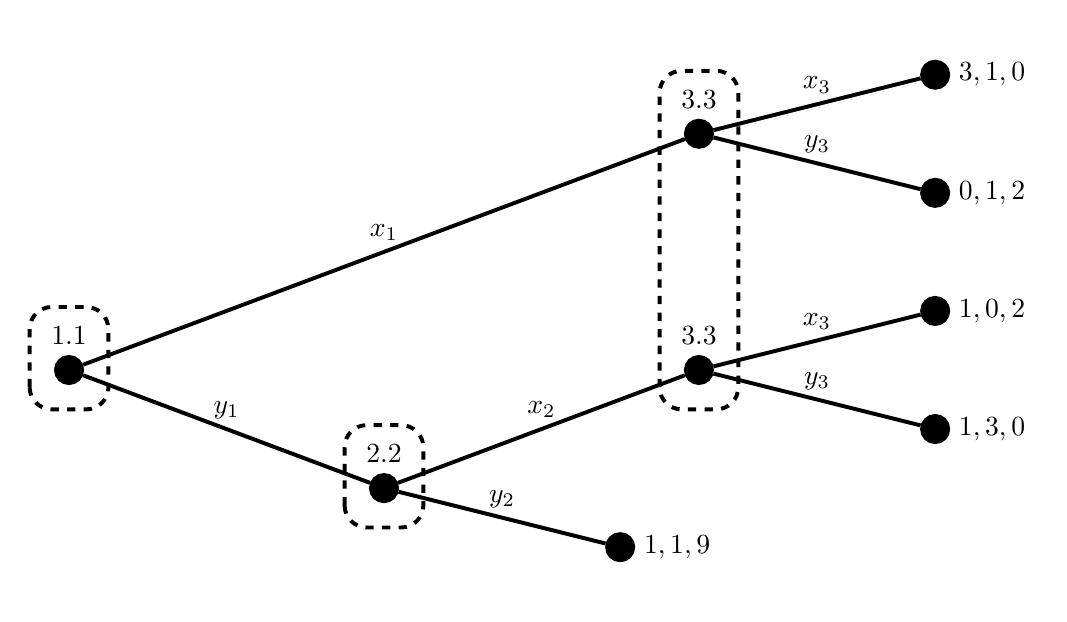
\begin{tikzpicture}[scale=2,looseness=.8,auto]
	\begin{scope}[every node/.style={font=\small\itshape},line width=0.5mm]
		\tikzstyle{every node}=[draw,fill=black,shape=circle,line width=0.5mm,minimum size=1.5mm,label distance=1mm];
		\path (0, 0   ) node (v11)  {} node [above,draw=none,fill=none] {$1.1$};
		\path (2,-0.75) node (v22)  {} node [above,draw=none,fill=none] {$2.2$};
		\path (4, 1.5 ) node (v33a) {} node [above,draw=none,fill=none] {$3.3$};
		\path (4, 0   ) node (v33b) {} node [above,draw=none,fill=none] {$3.3$};
		\path (5.5, 1.875) node (po1) {} node [right,draw=none,fill=none,xshift=1mm] {$3,1,0$};
		\path (5.5, 1.125) node (po2) {} node [right,draw=none,fill=none,xshift=1mm] {$0,1,2$};
		\path (5.5, 0.375) node (po3) {} node [right,draw=none,fill=none,xshift=1mm] {$1,0,2$};
		\path (5.5,-0.375) node (po4) {} node [right,draw=none,fill=none,xshift=1mm] {$1,3,0$};
		\path (3.5,-1.125) node (po5) {} node [right,draw=none,fill=none,xshift=1mm] {$1,1,9$};
		\draw (v11)  -- (v33a) node [midway,above,draw=none,fill=none,yshift=-1.5mm] {$x_1$};
		\draw (v11)  -- (v22)  node [midway,above,draw=none,fill=none,yshift=-1.5mm] {$y_1$};
		\draw (v22)  -- (v33b) node [midway,above,draw=none,fill=none,yshift=-1.5mm] {$x_2$};
		\draw (v33a) -- (po1)  node [midway,above,draw=none,fill=none,yshift=-1.5mm] {$x_3$};
		\draw (v33a) -- (po2)  node [midway,above,draw=none,fill=none,yshift=-1.5mm] {$y_3$};
		\draw (v33b) -- (po3)  node [midway,above,draw=none,fill=none,yshift=-1.5mm] {$x_3$};
		\draw (v33b) -- (po4)  node [midway,above,draw=none,fill=none,yshift=-1.5mm] {$y_3$};
		\draw (v22)  -- (po5)  node [midway,above,draw=none,fill=none,yshift=-1.5mm] {$y_2$};
		
		\draw[rounded corners=8pt,dashed] (-.25,-.25) rectangle (0.25,0.4);
		\draw[rounded corners=8pt,dashed] (1.75,-1) rectangle (2.25,-.35);
		\draw[rounded corners=8pt,dashed] (3.75,-.25) rectangle (4.25,1.9);
	\end{scope}
\end{tikzpicture}
\end{center}

\begin{enumerate}
	\item[a.] Show that this game has a unique equilibrium in behavioral strategy where Player~3 can actually play (because Player~1 plays $x_1$ or because Player~2 plays $x_2$).
	\item[b.] Now, assume that Players~1 and~2 do not have the same belief about the strategy that Player~3 would use if he was allowed to play. Show that in this case, Players~1 and~2 could behave rationally so that the probability that the Player~3 can move is zero.
\end{enumerate}

\nosolution

\end{document}
